% Options for packages loaded elsewhere
\PassOptionsToPackage{unicode}{hyperref}
\PassOptionsToPackage{hyphens}{url}
%
\documentclass[
  english,
  man]{apa6}
\usepackage{amsmath,amssymb}
\usepackage{lmodern}
\usepackage{ifxetex,ifluatex}
\ifnum 0\ifxetex 1\fi\ifluatex 1\fi=0 % if pdftex
  \usepackage[T1]{fontenc}
  \usepackage[utf8]{inputenc}
  \usepackage{textcomp} % provide euro and other symbols
\else % if luatex or xetex
  \usepackage{unicode-math}
  \defaultfontfeatures{Scale=MatchLowercase}
  \defaultfontfeatures[\rmfamily]{Ligatures=TeX,Scale=1}
\fi
% Use upquote if available, for straight quotes in verbatim environments
\IfFileExists{upquote.sty}{\usepackage{upquote}}{}
\IfFileExists{microtype.sty}{% use microtype if available
  \usepackage[]{microtype}
  \UseMicrotypeSet[protrusion]{basicmath} % disable protrusion for tt fonts
}{}
\makeatletter
\@ifundefined{KOMAClassName}{% if non-KOMA class
  \IfFileExists{parskip.sty}{%
    \usepackage{parskip}
  }{% else
    \setlength{\parindent}{0pt}
    \setlength{\parskip}{6pt plus 2pt minus 1pt}}
}{% if KOMA class
  \KOMAoptions{parskip=half}}
\makeatother
\usepackage{xcolor}
\IfFileExists{xurl.sty}{\usepackage{xurl}}{} % add URL line breaks if available
\IfFileExists{bookmark.sty}{\usepackage{bookmark}}{\usepackage{hyperref}}
\hypersetup{
  pdftitle={fractalRegression: An R package for multiscale regression and fractal analyses},
  pdfauthor={Aaron D. Likens1 \& Travis J. Wiltshire2},
  pdflang={en-EN},
  pdfkeywords={long range correlation, fractal, multiscale, dynamics},
  hidelinks,
  pdfcreator={LaTeX via pandoc}}
\urlstyle{same} % disable monospaced font for URLs
\usepackage{color}
\usepackage{fancyvrb}
\newcommand{\VerbBar}{|}
\newcommand{\VERB}{\Verb[commandchars=\\\{\}]}
\DefineVerbatimEnvironment{Highlighting}{Verbatim}{commandchars=\\\{\}}
% Add ',fontsize=\small' for more characters per line
\usepackage{framed}
\definecolor{shadecolor}{RGB}{248,248,248}
\newenvironment{Shaded}{\begin{snugshade}}{\end{snugshade}}
\newcommand{\AlertTok}[1]{\textcolor[rgb]{0.94,0.16,0.16}{#1}}
\newcommand{\AnnotationTok}[1]{\textcolor[rgb]{0.56,0.35,0.01}{\textbf{\textit{#1}}}}
\newcommand{\AttributeTok}[1]{\textcolor[rgb]{0.77,0.63,0.00}{#1}}
\newcommand{\BaseNTok}[1]{\textcolor[rgb]{0.00,0.00,0.81}{#1}}
\newcommand{\BuiltInTok}[1]{#1}
\newcommand{\CharTok}[1]{\textcolor[rgb]{0.31,0.60,0.02}{#1}}
\newcommand{\CommentTok}[1]{\textcolor[rgb]{0.56,0.35,0.01}{\textit{#1}}}
\newcommand{\CommentVarTok}[1]{\textcolor[rgb]{0.56,0.35,0.01}{\textbf{\textit{#1}}}}
\newcommand{\ConstantTok}[1]{\textcolor[rgb]{0.00,0.00,0.00}{#1}}
\newcommand{\ControlFlowTok}[1]{\textcolor[rgb]{0.13,0.29,0.53}{\textbf{#1}}}
\newcommand{\DataTypeTok}[1]{\textcolor[rgb]{0.13,0.29,0.53}{#1}}
\newcommand{\DecValTok}[1]{\textcolor[rgb]{0.00,0.00,0.81}{#1}}
\newcommand{\DocumentationTok}[1]{\textcolor[rgb]{0.56,0.35,0.01}{\textbf{\textit{#1}}}}
\newcommand{\ErrorTok}[1]{\textcolor[rgb]{0.64,0.00,0.00}{\textbf{#1}}}
\newcommand{\ExtensionTok}[1]{#1}
\newcommand{\FloatTok}[1]{\textcolor[rgb]{0.00,0.00,0.81}{#1}}
\newcommand{\FunctionTok}[1]{\textcolor[rgb]{0.00,0.00,0.00}{#1}}
\newcommand{\ImportTok}[1]{#1}
\newcommand{\InformationTok}[1]{\textcolor[rgb]{0.56,0.35,0.01}{\textbf{\textit{#1}}}}
\newcommand{\KeywordTok}[1]{\textcolor[rgb]{0.13,0.29,0.53}{\textbf{#1}}}
\newcommand{\NormalTok}[1]{#1}
\newcommand{\OperatorTok}[1]{\textcolor[rgb]{0.81,0.36,0.00}{\textbf{#1}}}
\newcommand{\OtherTok}[1]{\textcolor[rgb]{0.56,0.35,0.01}{#1}}
\newcommand{\PreprocessorTok}[1]{\textcolor[rgb]{0.56,0.35,0.01}{\textit{#1}}}
\newcommand{\RegionMarkerTok}[1]{#1}
\newcommand{\SpecialCharTok}[1]{\textcolor[rgb]{0.00,0.00,0.00}{#1}}
\newcommand{\SpecialStringTok}[1]{\textcolor[rgb]{0.31,0.60,0.02}{#1}}
\newcommand{\StringTok}[1]{\textcolor[rgb]{0.31,0.60,0.02}{#1}}
\newcommand{\VariableTok}[1]{\textcolor[rgb]{0.00,0.00,0.00}{#1}}
\newcommand{\VerbatimStringTok}[1]{\textcolor[rgb]{0.31,0.60,0.02}{#1}}
\newcommand{\WarningTok}[1]{\textcolor[rgb]{0.56,0.35,0.01}{\textbf{\textit{#1}}}}
\usepackage{longtable,booktabs,array}
\usepackage{calc} % for calculating minipage widths
% Correct order of tables after \paragraph or \subparagraph
\usepackage{etoolbox}
\makeatletter
\patchcmd\longtable{\par}{\if@noskipsec\mbox{}\fi\par}{}{}
\makeatother
% Allow footnotes in longtable head/foot
\IfFileExists{footnotehyper.sty}{\usepackage{footnotehyper}}{\usepackage{footnote}}
\makesavenoteenv{longtable}
\usepackage{graphicx}
\makeatletter
\def\maxwidth{\ifdim\Gin@nat@width>\linewidth\linewidth\else\Gin@nat@width\fi}
\def\maxheight{\ifdim\Gin@nat@height>\textheight\textheight\else\Gin@nat@height\fi}
\makeatother
% Scale images if necessary, so that they will not overflow the page
% margins by default, and it is still possible to overwrite the defaults
% using explicit options in \includegraphics[width, height, ...]{}
\setkeys{Gin}{width=\maxwidth,height=\maxheight,keepaspectratio}
% Set default figure placement to htbp
\makeatletter
\def\fps@figure{htbp}
\makeatother
\setlength{\emergencystretch}{3em} % prevent overfull lines
\providecommand{\tightlist}{%
  \setlength{\itemsep}{0pt}\setlength{\parskip}{0pt}}
\setcounter{secnumdepth}{-\maxdimen} % remove section numbering
% Make \paragraph and \subparagraph free-standing
\ifx\paragraph\undefined\else
  \let\oldparagraph\paragraph
  \renewcommand{\paragraph}[1]{\oldparagraph{#1}\mbox{}}
\fi
\ifx\subparagraph\undefined\else
  \let\oldsubparagraph\subparagraph
  \renewcommand{\subparagraph}[1]{\oldsubparagraph{#1}\mbox{}}
\fi
% Manuscript styling
\usepackage{upgreek}
\captionsetup{font=singlespacing,justification=justified}

% Table formatting
\usepackage{longtable}
\usepackage{lscape}
% \usepackage[counterclockwise]{rotating}   % Landscape page setup for large tables
\usepackage{multirow}		% Table styling
\usepackage{tabularx}		% Control Column width
\usepackage[flushleft]{threeparttable}	% Allows for three part tables with a specified notes section
\usepackage{threeparttablex}            % Lets threeparttable work with longtable

% Create new environments so endfloat can handle them
% \newenvironment{ltable}
%   {\begin{landscape}\centering\begin{threeparttable}}
%   {\end{threeparttable}\end{landscape}}
\newenvironment{lltable}{\begin{landscape}\centering\begin{ThreePartTable}}{\end{ThreePartTable}\end{landscape}}

% Enables adjusting longtable caption width to table width
% Solution found at http://golatex.de/longtable-mit-caption-so-breit-wie-die-tabelle-t15767.html
\makeatletter
\newcommand\LastLTentrywidth{1em}
\newlength\longtablewidth
\setlength{\longtablewidth}{1in}
\newcommand{\getlongtablewidth}{\begingroup \ifcsname LT@\roman{LT@tables}\endcsname \global\longtablewidth=0pt \renewcommand{\LT@entry}[2]{\global\advance\longtablewidth by ##2\relax\gdef\LastLTentrywidth{##2}}\@nameuse{LT@\roman{LT@tables}} \fi \endgroup}

% \setlength{\parindent}{0.5in}
% \setlength{\parskip}{0pt plus 0pt minus 0pt}

% \usepackage{etoolbox}
\makeatletter
\patchcmd{\HyOrg@maketitle}
  {\section{\normalfont\normalsize\abstractname}}
  {\section*{\normalfont\normalsize\abstractname}}
  {}{\typeout{Failed to patch abstract.}}
\patchcmd{\HyOrg@maketitle}
  {\section{\protect\normalfont{\@title}}}
  {\section*{\protect\normalfont{\@title}}}
  {}{\typeout{Failed to patch title.}}
\makeatother
\shorttitle{FRACTAL REGRESSION}
\keywords{long range correlation, fractal, multiscale, dynamics\newline\indent Word count: X}
\DeclareDelayedFloatFlavor{ThreePartTable}{table}
\DeclareDelayedFloatFlavor{lltable}{table}
\DeclareDelayedFloatFlavor*{longtable}{table}
\makeatletter
\renewcommand{\efloat@iwrite}[1]{\immediate\expandafter\protected@write\csname efloat@post#1\endcsname{}}
\makeatother
\usepackage{lineno}

\linenumbers
\usepackage{csquotes}
\ifxetex
  % Load polyglossia as late as possible: uses bidi with RTL langages (e.g. Hebrew, Arabic)
  \usepackage{polyglossia}
  \setmainlanguage[]{english}
\else
  \usepackage[main=english]{babel}
% get rid of language-specific shorthands (see #6817):
\let\LanguageShortHands\languageshorthands
\def\languageshorthands#1{}
\fi
\ifluatex
  \usepackage{selnolig}  % disable illegal ligatures
\fi
\newlength{\cslhangindent}
\setlength{\cslhangindent}{1.5em}
\newlength{\csllabelwidth}
\setlength{\csllabelwidth}{3em}
\newenvironment{CSLReferences}[2] % #1 hanging-ident, #2 entry spacing
 {% don't indent paragraphs
  \setlength{\parindent}{0pt}
  % turn on hanging indent if param 1 is 1
  \ifodd #1 \everypar{\setlength{\hangindent}{\cslhangindent}}\ignorespaces\fi
  % set entry spacing
  \ifnum #2 > 0
  \setlength{\parskip}{#2\baselineskip}
  \fi
 }%
 {}
\usepackage{calc}
\newcommand{\CSLBlock}[1]{#1\hfill\break}
\newcommand{\CSLLeftMargin}[1]{\parbox[t]{\csllabelwidth}{#1}}
\newcommand{\CSLRightInline}[1]{\parbox[t]{\linewidth - \csllabelwidth}{#1}\break}
\newcommand{\CSLIndent}[1]{\hspace{\cslhangindent}#1}

\title{fractalRegression: An R package for multiscale regression and fractal analyses}
\author{Aaron D. Likens\textsuperscript{1} \& Travis J. Wiltshire\textsuperscript{2}}
\date{}


\authornote{

Add complete departmental affiliations for each author here. Each new line herein must be indented, like this line.
Enter author note here.

The authors made the following contributions. Aaron D. Likens: Conceptualization, Software, Writing - Original Draft Preparation, Writing - Review \& Editing; Travis J. Wiltshire: Writing - Original Draft Preparation, Writing - Review \& Editing, Software.

Correspondence concerning this article should be addressed to Aaron D. Likens, Postal address. E-mail: \href{mailto:alikens@unomaha.edu}{\nolinkurl{alikens@unomaha.edu}}

}

\affiliation{\vspace{0.5cm}\textsuperscript{1} Department of Biomechanics, University of Nebraska at Omaha\\\textsuperscript{2} Department of Cognitive Science \& Artificial Intelligence, Tilburg University}

\abstract{
Time series data from scientific fields as diverse as astrophysics, economics, human movement science, and neuroscience all exhibit fractal properties. That is, these time series often exhibit self-similarity and long-range correlations. This \texttt{fractalRegression} package implements a number of univariate and bivariate time series tools appropriate for analyzing noisy data exhibiting these properties. These methods, especially the bivariate tools (Kristoufek, 2015a; Likens, Amazeen, West, \& Gibbons, 2019) have yet to be implemented in an open source and complete package for the R Statistical Software environment. As both practitioners and developers of these methods, we expect these tools will be of interest to a wide audience of scientists who use R, especially those from fields such as the human movement, cognitive, and other behavioral sciences. The algorithms have been developed in C++ using the popular Rcpp (Eddelbuettel \& Francois, 2011) and RcppArmadillo (Eddelbuettel \& Sanderson, 2014) packages. The result is a collection of efficient functions that perform well even on long time series (e.g., \(\geq\) 10,000 data points). In this work, we motivate introduce the package, each of the functions, and give examples of their use as well as issues to consider to correctly use these methods.
}



\begin{document}
\maketitle

\hypertarget{introduction}{%
\section{Introduction}\label{introduction}}

Fractal analysis, in its many forms, has become an important framework
in virtually every area of science, often serving as an indicator of
system health (Goldberger et al., 2002), adaptability
(Bak, Tang, \& Wiesenfeld, 1987), control
(Likens, Fine, Amazeen, \& Amazeen, 2015), cognitive function
(Euler, Wiltshire, Niermeyer, \& Butner, 2016), and multi-scale interactions
(Kelty-Stephen, 2017). In particular, various
methods related to Detrended Fluctuation Analysis (DFA)
(Peng et al., 1994) have rose to prominence due to their
ease of understanding and broad applicability to stationary and
nonstationary time series, alike.

The basic DFA algorithm has been implemented in numerous packages and
software programs. However, advanced methods such as Multifractal
Detrended Fluctuation Analysis (MFDFA)
(Kantelhardt et al., 2002), Detrended Cross
Correlation (DCCA) (Podobnik \& Stanley, 2008; Zebende, 2011), and, in particular,
fractal regression techniques such as Multiscale Regression Analysis
(MRA) (Kristoufek, 2015a; Likens, Amazeen, West, \& Gibbons, 2019) have not yet been
implemented in a comprehensive CRAN Package for the R Statistical
Software Environment. Thus, there is a clear need for a package that
incorporates this functionality in order to advance theoretical research
focused on understanding the time varying properties of natural
phenomena and applied research that uses those insights in important
areas such as healthcare (Cavanaugh, Kelty-Stephen, \& Stergiou, 2017) and education (Snow, Likens, Allen, \& McNamara, 2016).

\hypertarget{package-overview}{%
\section{Package Overview}\label{package-overview}}

Some foundational efforts in fractal analyses, which partially overlap
with the functionality of this package, have been implemented elsewhere.
For example, a number of univariate fractal and multifractal analyses
have been implemented in the `fracLab' library for MATLAB (Legrand \& Véhel, 2003)
and other toolboxes that are mainly targeted at multifractal analysis
(Ihlen, 2012; Ihlen \& Vereijken, 2010). In terms of
open access packages, there are other packages that implement some, but
not all of the same functions such as the \texttt{fathon} package
(Bianchi, 2020) that has been implemented in Python as well as the R
packages: \texttt{fractal} {[}defunct{]}, \texttt{nonlinearTseries}
(Garcia, 2020), and \texttt{MFDFA}
(Laib, Golay, Telesca, \& Kanevski, 2018). However, none of the above packages
incorporate univariate monofractal and multifractal DFA with bivariate
DCCA and MRA nor do they run on a C++ architecture. Our
\texttt{fractalRegression} package is unique in this combination of analyses
and efficiency. For instance, we are not aware of any other packages
that feature MRA and Multiscale Lagged Regression (MLRA).

\hypertarget{methodological-details-and-examples}{%
\section{Methodological Details and Examples}\label{methodological-details-and-examples}}

In order to demonstrate the methods within the `fractalRegression'
package, we group this into univariate (DFA, MFDFA) and bivariate
methods (DCCA, MRA, MRLA). For each method, we 1) highlight the key
question(s) that can be answered with that method, 2) briefly describe
the algorithm with sources for additional details, 3) describe some key
consideration for appropriately applying the algorithm, and demonstrate
the use of the functions on a 4) simulated and 5) empirical application
of the function. An overview of the functions included in the package,
the general objective of that function, and the output are shown below
in Table 1. The additional details are included in the sections
corresponding to those methods, in the package documentation, and in the
original sources for the methods.

\textbf{Table 1.}

\emph{Overview of package functions, objectives, and output}

\begin{longtable}[]{@{}
  >{\raggedright\arraybackslash}p{(\columnwidth - 4\tabcolsep) * \real{0.11}}
  >{\raggedright\arraybackslash}p{(\columnwidth - 4\tabcolsep) * \real{0.21}}
  >{\raggedright\arraybackslash}p{(\columnwidth - 4\tabcolsep) * \real{0.31}}@{}}
\toprule
Fun
ction & Objective & Output \\
\midrule
\endhead
dfa & Estimate
long-range
correlation
in a time
series & Object containing
the overall
\(\alpha\) estimate
and, if desired the
\texttt{logScales} and
\texttt{logRMS} \\
mfdfa & Estimate the
magnitude
and range of
long-range
correlations
in a time
series & Object containing
the \(\log_2\) scales
used for the
analysis, the
\(\log_2\)
fluctuation
function for each
scale and \(q\), the
various q-order
exponents, \(Hq\),
\(Tau\), \(h\), and
\(Dh\) \\
dcca & Estimates of
sc
ale-specific
correlation
between two
time-series & Object containing
the scales used for
the analysis and
the \(\rho\) '\texttt{rho\textquotesingle{}}
values for each
scale \\
mra & Estimates
the scale
specific
regression
coefficients
for a
predictor
time series
on and
outcome time
series & Object containing
the scales and
scale specific
\(\beta\) estimates,
\(R^2\), and \(t\)
statistics \\
mlra & Estimates
the scale
specific
regression
coefficients
for a
predictor
time series
on and
outcome time
series at
p
re-specified
lags & Object with
lag-specific
\(\beta\)
coefficients \\
fg
n\_sim & Simulate
fractional
Gaussian
noise & Returns a vector of
length \texttt{n}
according to the
specified \texttt{H} Hurst
exponent \\
iaaft & Generate
surrogate
series using
the
iterative
amplitude
adjusted
Fourier
transform & Returns a vector of
same length as
input time series \\
\bottomrule
\end{longtable}

\hypertarget{univariate-methods}{%
\subsection{Univariate Methods}\label{univariate-methods}}

\hypertarget{detrended-fluctuation-analysis}{%
\subsubsection{Detrended Fluctuation Analysis}\label{detrended-fluctuation-analysis}}

The key question that can be answered by Detrended Fluctuation Analysis
(DFA) (Peng et al., 1994) is: \emph{what is the magnitude and
direction of long range correlation in a single time series?} While DFA
has been described extensively elsewhere
(Kantelhardt, Koscielny-Bunde, Rego, Havlin, \& Bunde, 2001) and visualized nicely
(Kelty-Stephen, Stirling, \& Lipsitz, 2016), we provide a brief
summary here. DFA entails splitting a time series into several small
bins (e.g., 16). In each bin, the least squares regression is fit and
subtracted within each window. Residuals are squared and averaged within
each window. Then, the square root is taken of the average squared
residual across all windows of a given size. This process repeats for
larger window sizes, growing by, say a power of 2, up to N/4, where N is
the length of the series. In a final step, the logarithm of those scaled
root mean squared residuals (i.e., fluctuations) is regressed on the
logarithm of window sizes. The slope of this line is termed \(\alpha\) and
it provides a measure of the long range correlation. \(\alpha\) is
commonly used an as estimator of the Hurst exponent (H), where
\(\alpha<1\) = \(H\), and for \(\alpha>1\), \(H = 1 - \alpha\). Conventional
interpretation of \(\alpha\) is: \(\alpha < 0.5\) is anti-correlated,
\(\alpha ~= 0.5\) is uncorrelated, white noise, \(\alpha > 0.5\) is
temporally correlated, \(\alpha ~= 1\) is long-range correlated,
1/f-noise, pink noise, \(\alpha > 1\) is non-stationary and unbounded, and
\(\alpha ~= 1.5\) is fractional brownian motion.

\hypertarget{dfa-examples}{%
\paragraph{DFA Examples}\label{dfa-examples}}

To demonstrate the use of \texttt{dfa()} we simulate three time series using
the \texttt{fgn\_sim()} function. This is a simple function based on the former
\texttt{fARMA} R package. It only requires the number of observations \texttt{n}, and
the Hurst exponent \texttt{H}. In particular, we simulate white noise, pink
noise, and anti-correlated fractional Gaussian noise using the code
below.

\begin{Shaded}
\begin{Highlighting}[]
\NormalTok{white.noise }\OtherTok{\textless{}{-}} \FunctionTok{rnorm}\NormalTok{(}\DecValTok{5000}\NormalTok{)}
\NormalTok{pink.noise }\OtherTok{\textless{}{-}} \FunctionTok{fgn\_sim}\NormalTok{(}\AttributeTok{n =} \DecValTok{5000}\NormalTok{, }\AttributeTok{H =} \FloatTok{0.9}\NormalTok{)}
\NormalTok{anti.corr.noise }\OtherTok{\textless{}{-}} \FunctionTok{fgn\_sim}\NormalTok{(}\DecValTok{5000}\NormalTok{, }\AttributeTok{H =} \FloatTok{0.25}\NormalTok{)}
\end{Highlighting}
\end{Shaded}

Then we can run DFA on these using the example code below. Note that
this example uses a linear detrending with minimum scale (\texttt{sc\_min}) of
16, a maximum scale (\texttt{sc\_max}) of 1/4 the time series length, and
logarithmically spaced scale factor (\texttt{scale\_ratio}) of 2.

\begin{Shaded}
\begin{Highlighting}[]
\NormalTok{dfa.white }\OtherTok{\textless{}{-}} \FunctionTok{dfa}\NormalTok{(}\AttributeTok{x =}\NormalTok{ white.noise, }\AttributeTok{order =} \DecValTok{1}\NormalTok{, }\AttributeTok{verbose =} \DecValTok{1}\NormalTok{,}
                \AttributeTok{sc\_min =} \DecValTok{16}\NormalTok{, }\AttributeTok{sc\_max =} \FunctionTok{length}\NormalTok{(pink.noise)}\SpecialCharTok{/}\DecValTok{4}\NormalTok{, }\AttributeTok{scale\_ratio =} \DecValTok{2}\NormalTok{)}
\NormalTok{dfa.pink }\OtherTok{\textless{}{-}} \FunctionTok{dfa}\NormalTok{(}\AttributeTok{x =}\NormalTok{ pink.noise, }\AttributeTok{order =} \DecValTok{1}\NormalTok{, }\AttributeTok{verbose =} \DecValTok{1}\NormalTok{,}
                \AttributeTok{sc\_min =} \DecValTok{16}\NormalTok{, }\AttributeTok{sc\_max =} \FunctionTok{length}\NormalTok{(pink.noise)}\SpecialCharTok{/}\DecValTok{4}\NormalTok{, }\AttributeTok{scale\_ratio =} \DecValTok{2}\NormalTok{)}
\NormalTok{dfa.anti.corr }\OtherTok{\textless{}{-}} \FunctionTok{dfa}\NormalTok{(}\AttributeTok{x =}\NormalTok{ anti.corr.noise, }\AttributeTok{order =} \DecValTok{1}\NormalTok{, }\AttributeTok{verbose =} \DecValTok{1}\NormalTok{,}
                \AttributeTok{sc\_min =} \DecValTok{16}\NormalTok{, }\AttributeTok{sc\_max =} \FunctionTok{length}\NormalTok{(pink.noise)}\SpecialCharTok{/}\DecValTok{4}\NormalTok{, }\AttributeTok{scale\_ratio =} \DecValTok{2}\NormalTok{)}
\end{Highlighting}
\end{Shaded}

In terms of output from the above examples, for white noise, we observed
that \(\alpha\) = 0.52, for pink noise we observed that
\(\alpha\) = 0.91, and since we simulated anti-correlated
noise with H = 0.25, we observed a close estimate of the \(\alpha\) =
0.26. In terms of the objects saved from the \texttt{dfa()}
function, one commonly inspects the \texttt{logScales}-\texttt{logRms} plots. Given
the estimates above, we see in Figure 1 that the slopes for white noise,
pink noise, and anti-correlated noise conform to our expectations.

\textbf{Figure 1}

\emph{LogScale-LogFluctuation plots for white noise (left), pink noise
(middle), and anti-correlated noise (right)}

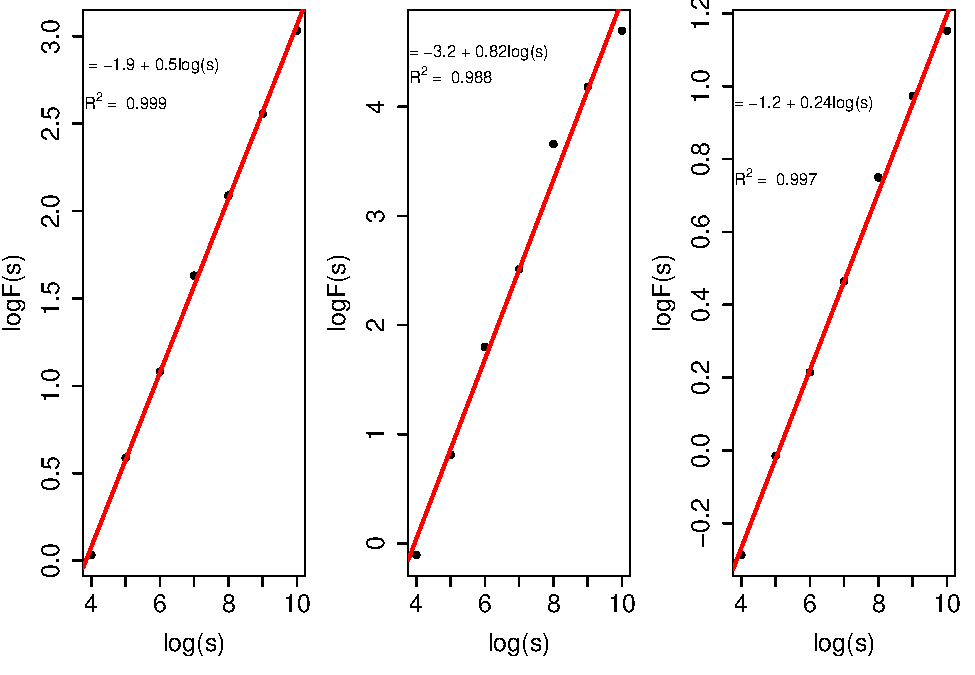
\includegraphics{fractal_regression_paper_brm_files/figure-latex/unnamed-chunk-3-1.pdf}

For an empirical example, we apply the \texttt{dfa()} function to DESCRIBE DATA
HERE. Movement Data?

\textbf{Figure 2}

\emph{LogScale-LogFluctuation plots for empirical time series (ADD ME)}

\hypertarget{multifractal-detrended-fluctuation-analysis}{%
\subsubsection{Multifractal Detrended Fluctuation Analysis}\label{multifractal-detrended-fluctuation-analysis}}

Multifractal Detrended Fluctuation Analysis (MFDFA;
Kantelhardt et al. (2002)) is an extension of DFA
by generalizing the fluctuation function to a range of exponents of the
qth order. The key question that can be answered by MFDFA is: \emph{how does
the magnitude and direction of long range correlation change over time
within a single time series?} Like DFA, MFDFA entails splitting a time
series into several small bins (e.g., 16). In each bin, the least
squares regression is fit and subtracted within each window. However,
the residuals are raised to a range of exponents \(q\) and averaged within
each window. So when \(q = 2\), DFA is equal to MFDFA. When \(q >2\), larger
residual are emphasized and when \(q < 2\), smaller residuals are
emphasized. The rest of the DFA algorithm is performed for each window
and windows size for all values of \(q\). We refer the reader to the work
of Kelty-Stephens and colleagues
Kelty-Stephen, Stirling, and Lipsitz (2016) Figure 3 for a
visualization of the algorithm and to Kantelhardt and colleagues
Kantelhardt et al. (2002) for additional
mathematical description.

\hypertarget{mfdfa-examples}{%
\subsubsection{MFDFA Examples}\label{mfdfa-examples}}

To demonstrate the use of \texttt{mfdfa()}, we work with data included in our
package (\texttt{fractaldata}), that was originally provided by
Ihlen (2012) . It includes a white noise
time series, monofractal time series, and a multifractal time series.
Investigation of the properties could also examine simulated
multifractal Brownian motion and multifractal Gaussian noise.

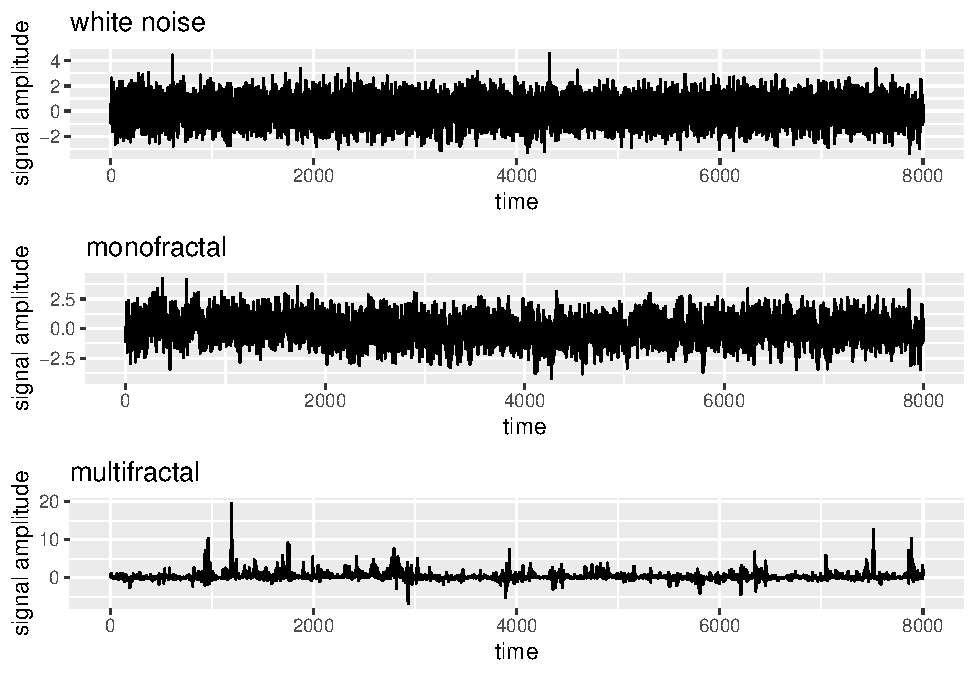
\includegraphics{fractal_regression_paper_brm_files/figure-latex/unnamed-chunk-4-1.pdf}

Simulated data: mfbrownian motion from Ihlen matlab (Aaron might have R
port) see mbm\_mgn for R from aaron - Empirical data: EPICLE Movement
Data?

\hypertarget{dfa-and-mfdfa-considerations}{%
\paragraph{DFA and MFDFA Considerations}\label{dfa-and-mfdfa-considerations}}

We recommend a few points of consideration here in using this function.
One is to be sure to verify there are not cross-over points in the
logScale-logFluctuation plots (Peng et al., 1994; Perakakis, Taylor, Martinez-Nieto, Revithi, \& Vila, 2009). Cross-over points (or a visible change in the slope as
a function of of scale) indicate that a mono-fractal characterization
does not sufficiently characterize the data. If cross-over points are
evident, we recommend proceeding to using the `mfdfa()' to estimate the
multi-fractal fluctuation dynamics across scales.

While it is common to use only linear detrending with DFA, it is
important to inspect the trends in the data to determine if it would be
more appropriate to use a higher order polynomial for detrending, and/or
compare the DFA output for different polynomial orders
(Kantelhardt, Koscielny-Bunde, Rego, Havlin, \& Bunde, 2001).

General recommendations for choosing the min and max scale are an sc\_min
= 10 and sc\_max = (N/4), where N is the number of observations. See Eke
et al.~(2002) (Eke, Herman, Kocsis, \& Kozak, 2002) and Gulich and
Zunino (2014) (Gulich \& Zunino, 2014) for additional
considerations.

\hypertarget{bivariate-methods}{%
\subsection{Bivariate Methods}\label{bivariate-methods}}

\hypertarget{detrended-cross-correlation-analysis}{%
\subsubsection{Detrended Cross-Correlation Analysis}\label{detrended-cross-correlation-analysis}}

Detrended Cross-Correlation Analysis (DCCA;
Podobnik and Stanley (2008)) is a bivariate extension
of the DFA algorithm generalizing it to a correlational case between two
time series. The key questions that can be asked it are: a) \emph{How does
correlation between two time series change as a function of scale?} and
b) \emph{What is/are the dominant (time) scale(s) of coordination? (those
that are beyond a threshold, or statistically significant given a
criteria, or of a certain magnitude?} For DCCA, the DFA algorithm gets
applied to both time series providing the scale-wise estimates for both.
DESCRIBE DCCA ALGORITHM HERE.

\hypertarget{dcca-examples}{%
\paragraph{DCCA Examples}\label{dcca-examples}}

\begin{itemize}
\item
  \begin{itemize}
  \tightlist
  \item
    Simulated data: MC-ARFIMA
  \item
    Empirical data: EPICLE Movement Data?
  \end{itemize}
\end{itemize}

\hypertarget{multi-scale-regression-analysis}{%
\subsubsection{Multi-scale Regression Analysis}\label{multi-scale-regression-analysis}}

Multi-scale regression analysis (MRA) is an adaptation of DCCA that
brings the analyses into a predictive, regression framework
Kristoufek (2015b) . The key questions that can be answered by it are: a)
\emph{How does the influence of one time series on another time series change
as a function of scale?} and b) \emph{What is/are the dominant (time)
scale(s) of influence of one time series on another time series?}
DESCRIBE MRA ALGORITHM HERE.

\hypertarget{mra-examples}{%
\paragraph{MRA Examples}\label{mra-examples}}

\begin{itemize}
\item
  MRA

  \begin{itemize}
  \tightlist
  \item
    Simulated data:
  \item
    Empirical data: FNIRS from Aaron?
  \end{itemize}
\end{itemize}

\hypertarget{multi-scale-lagged-regression-analysis}{%
\subsubsection{Multi-scale Lagged Regression Analysis}\label{multi-scale-lagged-regression-analysis}}

Multi-scale lagged regression analysis is an extension of MRA that
allows for examining the influence as a function of scale, but also of
time lag. In parituclar, the key questions that can be asked with MLRA
are: a) \emph{How does the influence of one time series on another time
series change as a function of scale at different time lags?} and b)
\emph{Does the dominant time scale of influence change over successive time
lags?} DESCRIBE MLRA ALGORITHM HERE.

\hypertarget{mlra-examples}{%
\paragraph{MLRA Examples}\label{mlra-examples}}

\begin{itemize}
\item
  MLRA

  \begin{itemize}
  \tightlist
  \item
    Key Question
  \item
    Simulated data: Equation from Aaron from grant on MLRA
  \item
    Empirical data: FNIRS from Aaron?
  \end{itemize}
\end{itemize}

\hypertarget{surrogate-methods-and-full-data-analysis}{%
\subsection{Surrogate Methods (and `full' data analysis)}\label{surrogate-methods-and-full-data-analysis}}

Methods are ranked in terms of increasing levels of rigor.

\begin{itemize}
\tightlist
\item
  Randomization - Estimates should be different.
\item
  IAAFT - Estimates should be different.
\item
  Model based surrogate (Simulated exponents) - See Likens 2019 paper
  with model of postural sway/control, taking an educated guess about
  the data generating process underlying the time series. Estimates
  should not be different. See Roume et al 2018 windowed detrended CCA
\item
  Can we incorporate lags into MC-ARFIMA?
\end{itemize}

\hypertarget{general-discussion}{%
\section{General Discussion}\label{general-discussion}}

\begin{itemize}
\tightlist
\item
  General value of methods and the types of questions
\item
  Practical consideration of univariate methods
\item
  Practical consideration of bivariate methods
\item
  Unique contribution of the methods
\end{itemize}

\hypertarget{acknowledgements}{%
\section{Acknowledgements}\label{acknowledgements}}

Author AL receives support from a National Institutes of Health Center
grant (P20GM109090).

\newpage

\hypertarget{references}{%
\section{References}\label{references}}

\begingroup
\setlength{\parindent}{-0.5in}
\setlength{\leftskip}{0.5in}

\hypertarget{refs}{}
\begin{CSLReferences}{1}{0}
\leavevmode\hypertarget{ref-bakSelforganizedCriticalityExplanation1987}{}%
Bak, P., Tang, C., \& Wiesenfeld, K. (1987). Self-organized criticality: {An} explanation of the 1/f noise. \emph{Physical Review Letters}, \emph{59}(4), 381--384. \url{https://doi.org/10.1103/PhysRevLett.59.381}

\leavevmode\hypertarget{ref-bianchi2020}{}%
Bianchi, S. (2020). Fathon: A python package for a fast computation of detrendend fluctuation analysis and related algorithms. \emph{Journal of Open Source Software}, \emph{5}(45), 1828.

\leavevmode\hypertarget{ref-cavanaugh2017}{}%
Cavanaugh, J. T., Kelty-Stephen, D. G., \& Stergiou, N. (2017). Multifractality, Interactivity, and the Adaptive Capacity of the Human Movement System: A Perspective for Advancing the Conceptual Basis of Neurologic Physical Therapy. Retrieved from \url{https://www.ingentaconnect.com/content/wk/npt/2017/00000041/00000004/art00007}

\leavevmode\hypertarget{ref-eddelbuettelRcppSeamlessIntegration2011}{}%
Eddelbuettel, D., \& Francois, R. (2011). Rcpp: {Seamless} {R} and {C}++ {Integration}. \emph{Journal of Statistical Software}, \emph{40}(1), 1--18. \url{https://doi.org/10.18637/jss.v040.i08}

\leavevmode\hypertarget{ref-eddelbuettelRcppArmadilloAcceleratingHighperformance2014}{}%
Eddelbuettel, D., \& Sanderson, C. (2014). {RcppArmadillo}: {Accelerating} {R} with high-performance {C}++~linear algebra. \emph{Computational Statistics \& Data Analysis}, \emph{71}, 1054--1063. \url{https://doi.org/10.1016/j.csda.2013.02.005}

\leavevmode\hypertarget{ref-ekeFractalCharacterizationComplexity2002}{}%
Eke, A., Herman, P., Kocsis, L., \& Kozak, L. R. (2002). Fractal characterization of complexity in temporal physiological signals. \emph{Physiological Measurement}, \emph{23}(1), R1--R38. \url{https://doi.org/10.1088/0967-3334/23/1/201}

\leavevmode\hypertarget{ref-eulerWorkingMemoryPerformance2016}{}%
Euler, M. J., Wiltshire, T. J., Niermeyer, M. A., \& Butner, J. E. (2016). Working memory performance inversely predicts spontaneous delta and theta-band scaling relations. \emph{Brain Research}, \emph{1637}, 22--33. \url{https://doi.org/10.1016/j.brainres.2016.02.008}

\leavevmode\hypertarget{ref-garciaNonlinearTseriesNonlinearTime2020}{}%
Garcia, C. A. (2020). {nonlinearTseries}: {Nonlinear} {Time} {Series} {Analysis}. Retrieved from \url{https://CRAN.R-project.org/package=nonlinearTseries}

\leavevmode\hypertarget{ref-goldbergerFractalDynamicsPhysiology2002}{}%
Goldberger, A. L., Amaral, L. A. N., Hausdorff, J. M., Ivanov, P. C., Peng, C.-K., \& Stanley, H. E. (2002). Fractal dynamics in physiology: {Alterations} with disease and aging. \emph{Proceedings of the National Academy of Sciences}, \emph{99}(suppl 1), 2466--2472. \url{https://doi.org/10.1073/pnas.012579499}

\leavevmode\hypertarget{ref-gulichCriterionDeterminationOptimal2014}{}%
Gulich, D., \& Zunino, L. (2014). A criterion for the determination of optimal scaling ranges in {DFA} and {MF}-{DFA}. \emph{Physica A: Statistical Mechanics and Its Applications}, \emph{397}, 17--30. \url{https://doi.org/10.1016/j.physa.2013.11.029}

\leavevmode\hypertarget{ref-ihlenIntroductionMultifractalDetrended2012}{}%
Ihlen, E. A. F. (2012). Introduction to {Multifractal} {Detrended} {Fluctuation} {Analysis} in {Matlab}. \emph{Frontiers in Physiology}, \emph{3}. \url{https://doi.org/10.3389/fphys.2012.00141}

\leavevmode\hypertarget{ref-ihlen2010}{}%
Ihlen, E. A. F., \& Vereijken, B. (2010). Interaction-dominant dynamics in human cognition: Beyond 1/{{}}? fluctuation. \emph{Journal of Experimental Psychology: General}, \emph{139}(3), 436--463. \url{https://doi.org/10.1037/a0019098}

\leavevmode\hypertarget{ref-kantelhardtDetectingLongrangeCorrelations2001}{}%
Kantelhardt, J. W., Koscielny-Bunde, E., Rego, H. H. A., Havlin, S., \& Bunde, A. (2001). Detecting long-range correlations with detrended fluctuation analysis. \emph{Physica A: Statistical Mechanics and Its Applications}, \emph{295}(3), 441--454. \url{https://doi.org/10.1016/S0378-4371(01)00144-3}

\leavevmode\hypertarget{ref-kantelhardtMultifractalDetrendedFluctuation2002}{}%
Kantelhardt, J. W., Zschiegner, S. A., Koscielny-Bunde, E., Havlin, S., Bunde, A., \& Stanley, H. E. (2002). Multifractal detrended fluctuation analysis of nonstationary time series. \emph{Physica A: Statistical Mechanics and Its Applications}, \emph{316}(1), 87--114. \url{https://doi.org/10.1016/S0378-4371(02)01383-3}

\leavevmode\hypertarget{ref-kelty-stephenThreadingMultifractalSocial2017}{}%
Kelty-Stephen, D. G. (2017). Threading a multifractal social psychology through within-organism coordination to within-group interactions: {A} tale of coordination in three acts. \emph{Chaos, Solitons \& Fractals}, \emph{104}, 363--370. \url{https://doi.org/10.1016/j.chaos.2017.08.037}

\leavevmode\hypertarget{ref-kelty-stephenMultifractalTemporalCorrelations2016}{}%
Kelty-Stephen, D. G., Stirling, L. A., \& Lipsitz, L. A. (2016). Multifractal temporal correlations in circle-tracing behaviors are associated with the executive function of rule-switching assessed by the {Trail} {Making} {Test}. \emph{Psychological Assessment}, \emph{28}(2), 171--180. \url{https://doi.org/10.1037/pas0000177}

\leavevmode\hypertarget{ref-kristoufekDetrendedFluctuationAnalysis2015}{}%
Kristoufek, L. (2015a). Detrended fluctuation analysis as a regression framework: {Estimating} dependence at different scales. \emph{Physical Review E}, \emph{91}(2), 022802. \url{https://doi.org/10.1103/PhysRevE.91.022802}

\leavevmode\hypertarget{ref-kristoufek2015}{}%
Kristoufek, L. (2015b). Detrended fluctuation analysis as a regression framework: Estimating dependence at different scales. \emph{Physical Review E}, \emph{91}(2), 022802. \url{https://doi.org/10.1103/PhysRevE.91.022802}

\leavevmode\hypertarget{ref-laibMultifractalAnalysisTime2018}{}%
Laib, M., Golay, J., Telesca, L., \& Kanevski, M. (2018). Multifractal analysis of the time series of daily means of wind speed in complex regions. \emph{Chaos, Solitons \& Fractals}, \emph{109}, 118--127. \url{https://doi.org/10.1016/j.chaos.2018.02.024}

\leavevmode\hypertarget{ref-legrand2003}{}%
Legrand, P., \& Véhel, J. L. (2003). Signal and image processing with FracLab. \emph{Thinking in Patterns: Fractals and Related Phenomena in Nature}, 321322.

\leavevmode\hypertarget{ref-likensStatisticalPropertiesMultiscale2019}{}%
Likens, A. D., Amazeen, P. G., West, S. G., \& Gibbons, C. T. (2019). Statistical properties of {Multiscale} {Regression} {Analysis}: {Simulation} and application to human postural control. \emph{Physica A: Statistical Mechanics and Its Applications}, \emph{532}, 121580. \url{https://doi.org/10.1016/j.physa.2019.121580}

\leavevmode\hypertarget{ref-likensExperimentalControlScaling2015}{}%
Likens, A. D., Fine, J. M., Amazeen, E. L., \& Amazeen, P. G. (2015). Experimental control of scaling behavior: What is not fractal? \emph{Experimental Brain Research}, \emph{233}(10), 2813--2821. \url{https://doi.org/10.1007/s00221-015-4351-4}

\leavevmode\hypertarget{ref-pengMosaicOrganizationDNA1994}{}%
Peng, C.-K., Buldyrev, S. V., Havlin, S., Simons, M., Stanley, H. E., \& Goldberger, A. L. (1994). Mosaic organization of {DNA} nucleotides. \emph{Physical Review E}, \emph{49}(2), 1685--1689. \url{https://doi.org/10.1103/PhysRevE.49.1685}

\leavevmode\hypertarget{ref-perakakis2009}{}%
Perakakis, P., Taylor, M., Martinez-Nieto, E., Revithi, I., \& Vila, J. (2009). Breathing frequency bias in fractal analysis of heart rate variability. \emph{Biological Psychology}, \emph{82}(1), 82--88. \url{https://doi.org/10.1016/j.biopsycho.2009.06.004}

\leavevmode\hypertarget{ref-podobnikDetrendedCrossCorrelationAnalysis2008}{}%
Podobnik, B., \& Stanley, H. E. (2008). Detrended {Cross}-{Correlation} {Analysis}: {A} {New} {Method} for {Analyzing} {Two} {Nonstationary} {Time} {Series}. \emph{Physical Review Letters}, \emph{100}(8), 084102. \url{https://doi.org/10.1103/PhysRevLett.100.084102}

\leavevmode\hypertarget{ref-snow2016}{}%
Snow, E. L., Likens, A. D., Allen, L. K., \& McNamara, D. S. (2016). Taking Control: Stealth Assessment of Deterministic Behaviors Within a Game-Based System. \emph{International Journal of Artificial Intelligence in Education}, \emph{26}(4), 1011--1032. \url{https://doi.org/10.1007/s40593-015-0085-5}

\leavevmode\hypertarget{ref-zebendeDCCACrosscorrelationCoefficient2011}{}%
Zebende, G. F. (2011). {DCCA} cross-correlation coefficient: {Quantifying} level of cross-correlation. \emph{Physica A: Statistical Mechanics and Its Applications}, \emph{390}(4), 614--618. \url{https://doi.org/10.1016/j.physa.2010.10.022}

\end{CSLReferences}

\endgroup


\end{document}
